\documentclass[12pt]{book}
\usepackage{diffyqssetupUB}

\begin{document}

{\color{teal}BH 20190729 diffyqssetup.sty and mywrapfig.sty 
both missing from Overleaf. In order to get this tex 
to compile on Overleaf, obtained missing sty files from Lebl's source, uploaded to Overleaf}
%extra material {Slope fields}

\subsection{Slope fields with Python}

The \emph{resources306} module provides a function \emph{slopefieldplot}.
You supply {\color{red}it} 
{\color{blue}\emph{slopefieldplot}} with a function {\color{blue}(called \emph{f} in the example below)} that returns the right hand side of your differential equation,
{\color{red}(called \emph{f} in the example below)} the desired minimum and maximum values on the horizontal and vertical axes respectively, and
the desired spacing between line segments on the horizontal axis. 
Any of the {\color{red}optional arguments} {\color{blue}graphical options} for \emph{matplotlib.pyplot.plot()}, such as line color, line width, etc., can also be supplied to \emph{slopefieldplot}.
Here we create a slope field plot for the differential equation $\frac{dy}{dx} = x^2 - y$:
\begin{small}
\begin{verbatim}
from resources306 import *
def f(x,y): return x**2 - y
slopefieldplot( f, -2,2, -1,2, .2 ,lw=2)
plt.xlabel('x')
plt.ylabel('y');
\end{verbatim}
\end{small}
{\color{blue}
If using a Python environment that does not automatically display graphics,
add the line "plt.show()".}

\noindent This generates the {\color{blue}slope field part} of the picture {\color{red}on the left} below.

%\parbox[c]{3.1in}{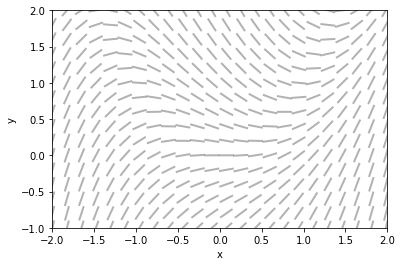
\includegraphics[width=3.0in]{additional_figures/First_order_ODEs__slopfieldplot}}
\parbox[c]{3.1in}{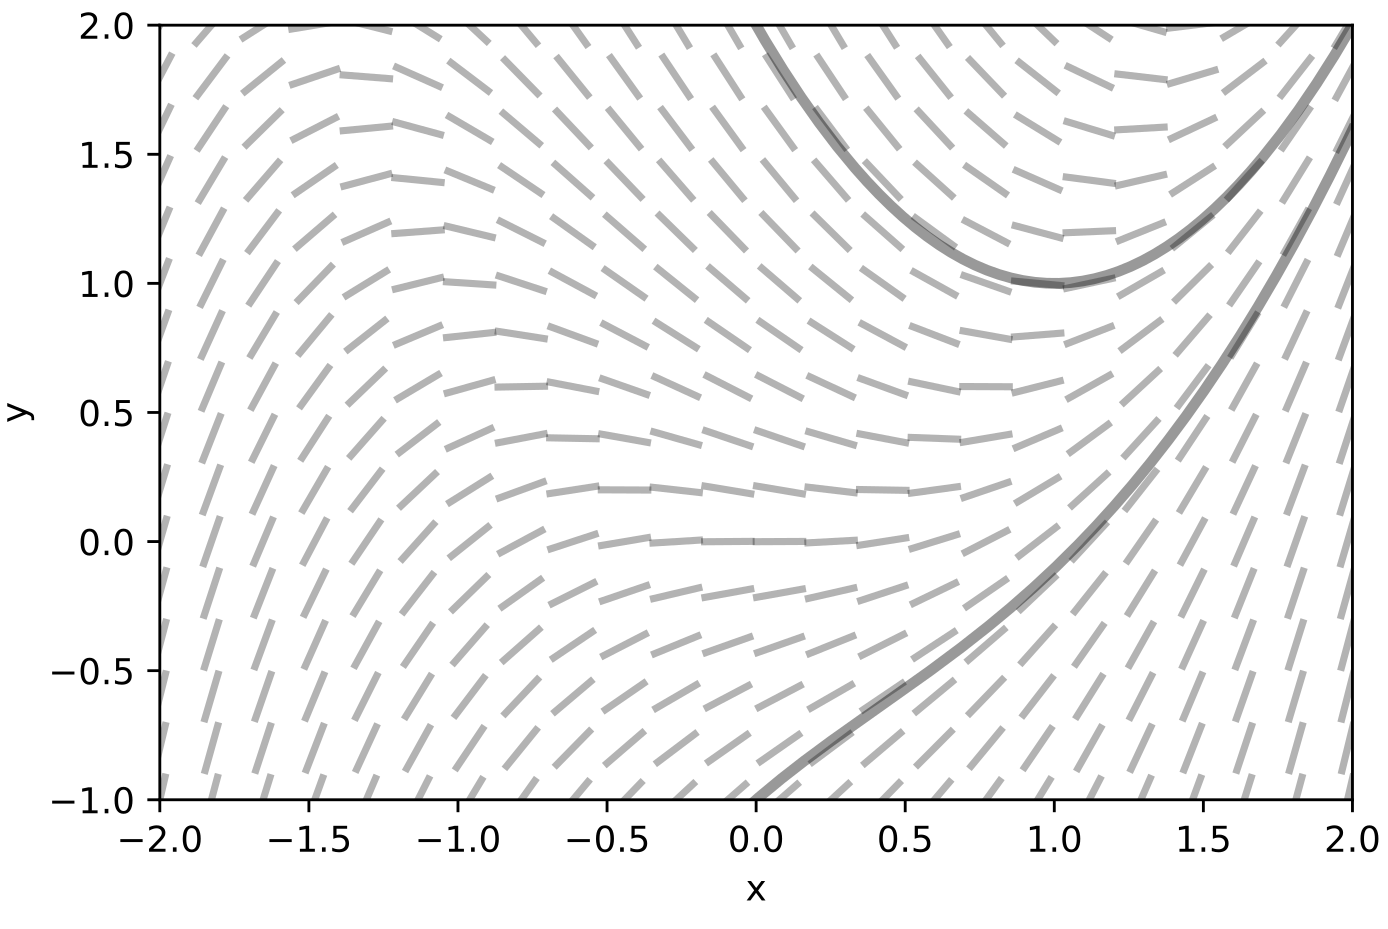
\includegraphics[width=5.0in]{additional_figures/First_order_ODEs__slopfieldplot_with_solutions}}

\noindent The \emph{resources306} module also provides a function \emph{expressionplot} as a simple way 
{\color{red}of creating a matplotlib plot of} 
{\color{blue}to plot} a sympy expression. 
{\color{red}It allows you, for example, to plot alleged solutions of a differential 
equation on top of its slope field.} 
You supply \emph{expressionplot} with the expression you want to plot, 
the (one and only) variable in the expression,
the minimum and maximum values of that variable to be shown in the plot, 
and any graphical options you like.
Below, we create two solutions of the differential equation $\frac{dy}{dx} = x^2 - y$ as sympy expressions:


\begin{small}
\begin{verbatim}
x = sp.symbols('x')
y1 = x**2-2*x+2
y2 = ((x**2-2*x+2)*sp.exp(x)-3)*sp.exp(-x)
y1,y2
\end{verbatim}
\end{small}
$$\left ( x^{2} - 2 x + 2, \quad \left(\left(x^{2} - 2 x + 2\right) e^{x} - 3\right) e^{- x}\right )$$

\noindent and then with the code below add their graphs to the slope field plot.
{\color{red}The result is the picture on the right above.}

\begin{small}
\begin{verbatim}
slopefieldplot( f, -2,2, -1,2, .2 ,lw=2)
expressionplot(y1,x,-2,2,color='r',alpha=.4,lw=3)
expressionplot(y2,x,-1,2,color='b',alpha=.4,lw=3)
plt.xlabel('x')
plt.ylabel('y')
\end{verbatim}
\end{small}
{\color{red}The result is the picture with two solution curves superimposed on a slope field.}

%extra exercises {Slope fields}

\begin{exercise}
Use the following method to determine $y(4)$ approximately if $y(0)=0$ and $\frac{dy}{dt} = \cos y + y \sin t$ for all $t$. {\color{green}JR The first sentence is pedagogically important. I want them to understand the goal from the outset, not to simply follow a set of instructions, wormlike.}
Use Python to draw the slope field of the differential equation on the region where $t$ runs from 0 to 5 and $y$ runs from -1 to 5. 
{\color{red}
(If you want to alter the size of the plot, you can use \emph{plt.figure(figsize=(W,H))}, where W and H are the width and height you want. }
Save the graphic you've created as a PNG image, and then open it in a program that
allows you to draw on it, like Inkscape, GIMP, etc.
On your slope field, sketch the curve $y(t)$ that has the following properties: (i) {\color{blue}$y(0)=0$,
i.e., it starts at $t=0$, $y=0$, (ii) its slope agrees with the slope field at every point along it.}
Then from your picture, estimate $y(4)$ as accurately as you can. {\color{green} JR Some BH changes reverted
for deliberate pedagogical reasons.}
\end{exercise}


%extra material {Numerical methods: Euler's method}

\subsection{Euler's method with Python}

Below we show an implementation of Euler's method applied to the 
initial value problem $y^\prime = x^2 - y$, $y(0)=2$. We plot the resulting Euler approximation on top of the slope field.

\begin{small}
\begin{verbatim}
from resources306 import *

def f(x,y): 
    return x**2 - y

plt.figure(figsize=(8,8))
slopefieldplot( f, 0,2.5, 0.5,3.5, .1 ,lw=2)

y = 2.0             # This is the initial value of y.
x = 0.0             # This is the initial time.
xfinal = 2.5        # This is the value of x we want to get to.
n = 8               # Here we say how many steps we want to take.
h =(xfinal-x)/n     # This is our step-size.

xlist = [x]         # Initialize lists to store the data in
ylist = [y]         # for later plotting.

for i in range(n):  # Take n steps
    slope = f(x,y)  # Compute the slope at the current location with DE
    y = y + h*slope # Take the Euler step to the new value of y.
    x = x + h       # Advance x by one step.
    xlist.append(x) # Tack the new values at the ends of the lists.
    ylist.append(y)

for x,y in zip(xlist,ylist):
    print(f'{x:8.4f} {y:12.8f}')

plt.plot( xlist, ylist, 'mo-', lw=3, alpha=0.6, label='Euler approximation' )
plt.xlabel('x')
plt.ylabel('y')
plt.grid()
plt.legend(loc='center')
\end{verbatim}
\end{small}

\begin{scriptsize}
\begin{verbatim}
  0.0000   2.00000000
  0.3125   1.37500000
  0.6250   0.97583008
  0.9375   0.79295349
  1.2500   0.81981373
  1.5625   1.05190319
  1.8750   1.48612290
  2.1875   2.12034230
  2.5000   2.95309666
\end{verbatim}
\end{scriptsize}

\parbox[c]{3.1in}{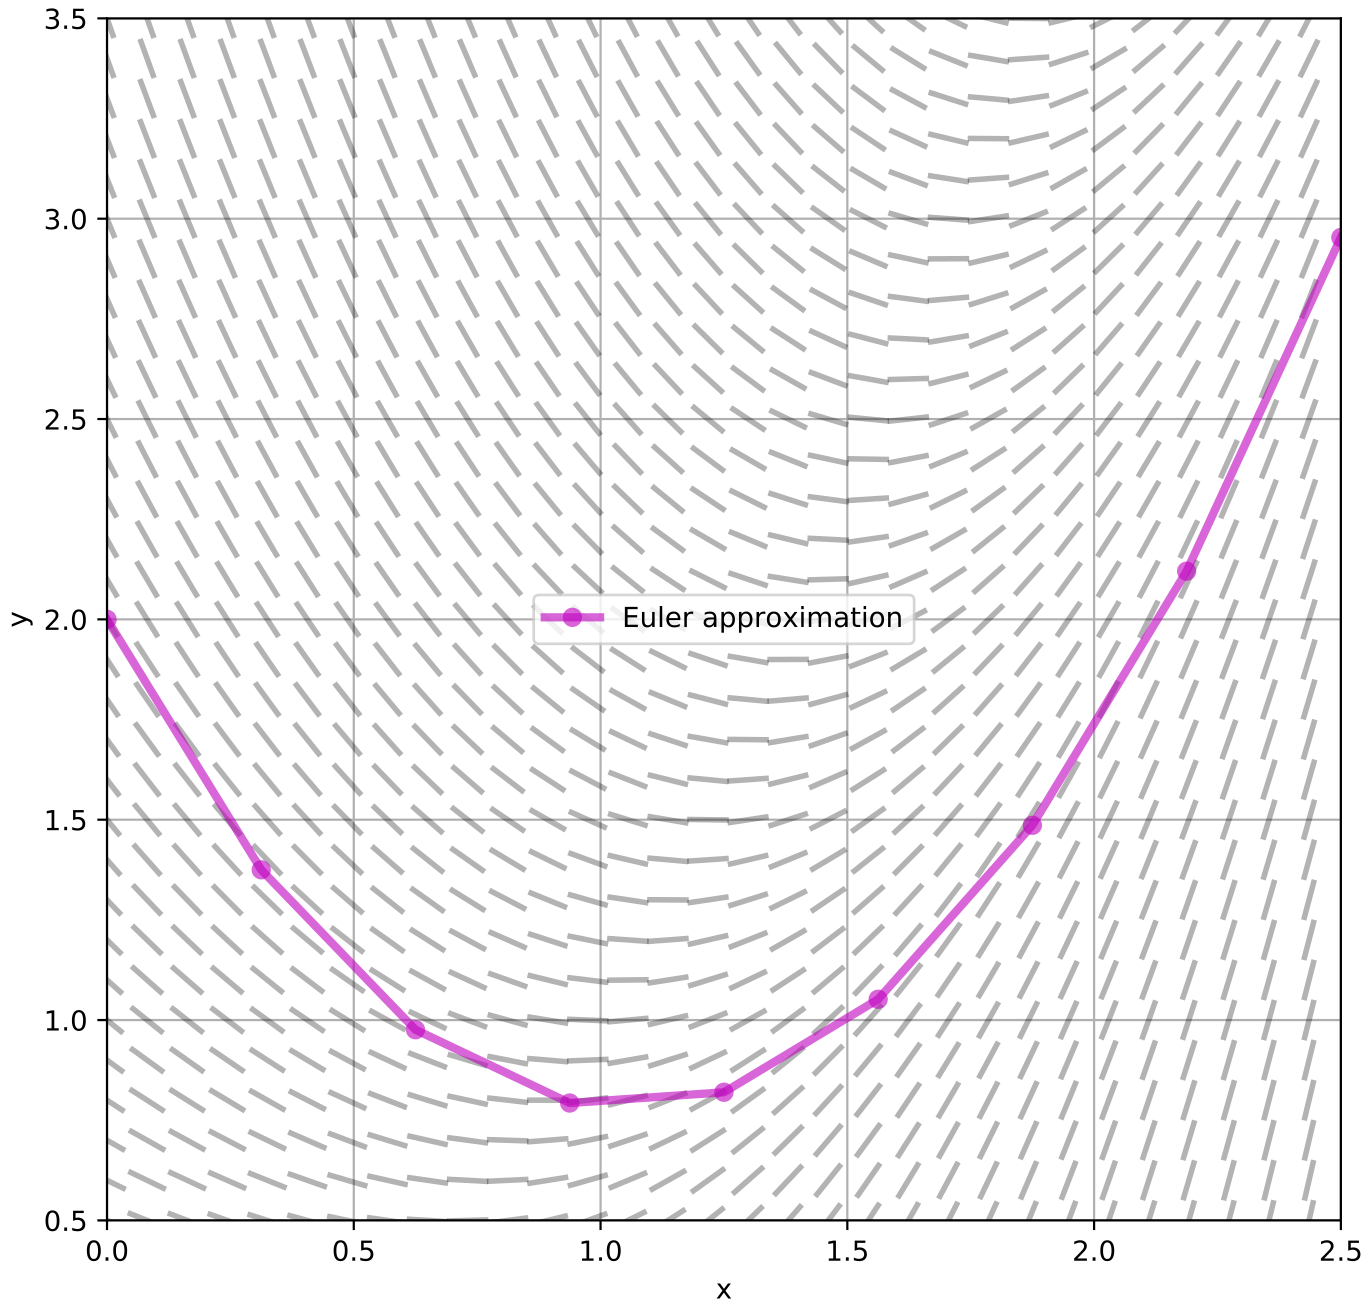
\includegraphics[width=5.0in]{additional_figures/First_order_ODEs__eulers_method_svg}}

{\color{green}BH In Euler's method code, 
xf suggests x for the function f.
Was the idea xfinal? JR Yes. I changed it to that.}

{\color{green}BH: Changed tiny to scriptsize (could be footnotesize) in output from Euler's method, changed width=3.0 to width=5.0 in includegraphics}
\end{document}

